\documentclass{beamer}
\usepackage[utf8]{inputenc}
\usepackage[czech, english]{babel}
\usepackage[IL2]{fontenc}
\usepackage{hyperref}
\usepackage{graphicx}

\usecolortheme{seahorse}
\usetheme{Antibes}

\title{Hloubkové vyhledávání v grafech}
\subtitle{Typografie a publikování --- 5.\, projekt}
\author{xplagiat0b}

\begin{document}

\frame{\titlepage}

\begin{frame}
    \frametitle{Obsah}
    \tableofcontents
\end{frame}

\section{Teorie}

\begin{frame}
    \frametitle{Vlastnosti}

    \begin{itemize}
        \item Časová složitost
        \item Prostorová složitost
        \item Kompletnost (pro konečné grafy)
    \end{itemize}

    \begin{block}{Hodnoty}
        \begin{itemize}
            \item Časová složitost: $O(n^m)$
            \item Prostorová složitost: $O(bm)$
            \item V obou případech je $m$ maximální možná hloubka jakéhokoli uzlu.
        \end{itemize}

    \end{block}

\end{frame}

\begin{frame}
    \frametitle{Využití}
    \begin{itemize}
        \item Nalezení cesty mezi dvěma uzly
        \item Zjištění acykličnosti grafu
        \item Nalezení silných komponent
        \item Topologické uspořádání uzlů grafu
        \item Určení následníka trůnu
    \end{itemize}

    \begin{alertblock}{Pozor}
        U většiny využití je základní algoritmus obohacen o další podmínky
    \end{alertblock}


\end{frame}

\section{Algoritmus}

\begin{frame}
    \frametitle{Základní popis}
    \begin{itemize}
        \item Využívá zásobník
        \item Zpracovává vždy uzel na vrcholu zásobníku.
        \item Po navštívení se na zásobník vloží všichni sousedé.
    \end{itemize}
\end{frame}

\begin{frame}
    \frametitle{Princip}
    \begin{itemize}
        \item Vloží počáteční uzel na zásobník
        \item Zpracuje uzel na vrchu zásobníku
        \item Vloží jeho potomky na zásobník
    \end{itemize}
\end{frame}

\begin{frame}
    \frametitle{Příklad}
    \begin{center}
        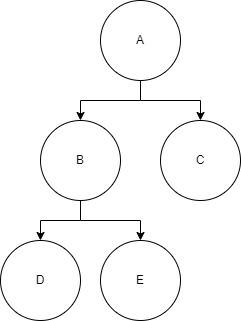
\includegraphics[totalheight=180pt, width=\textwidth, keepaspectratio]{dia.png}
    \end{center}
\end{frame}

\section{Zakončení}

\begin{frame}
    \frametitle{Použité zdroje}
    \begin{itemize}
        \item Uninformed Search Algorithms \\ \url{https://www.javatpoint.com/ai-uninformed-search-algorithms}
        \item Graph Algorithms \\ \url{https://www.javatpoint.com/graph-algorithms}
        \item
    \end{itemize}
\end{frame}

\begin{frame}

    \begin{center}
        \Large{Děkuji za pozornost.}
    \end{center}

\end{frame}

\end{document}
